\chapter*{Appendix}\label{chap:appendix}

\begin{figure}
	\centering
	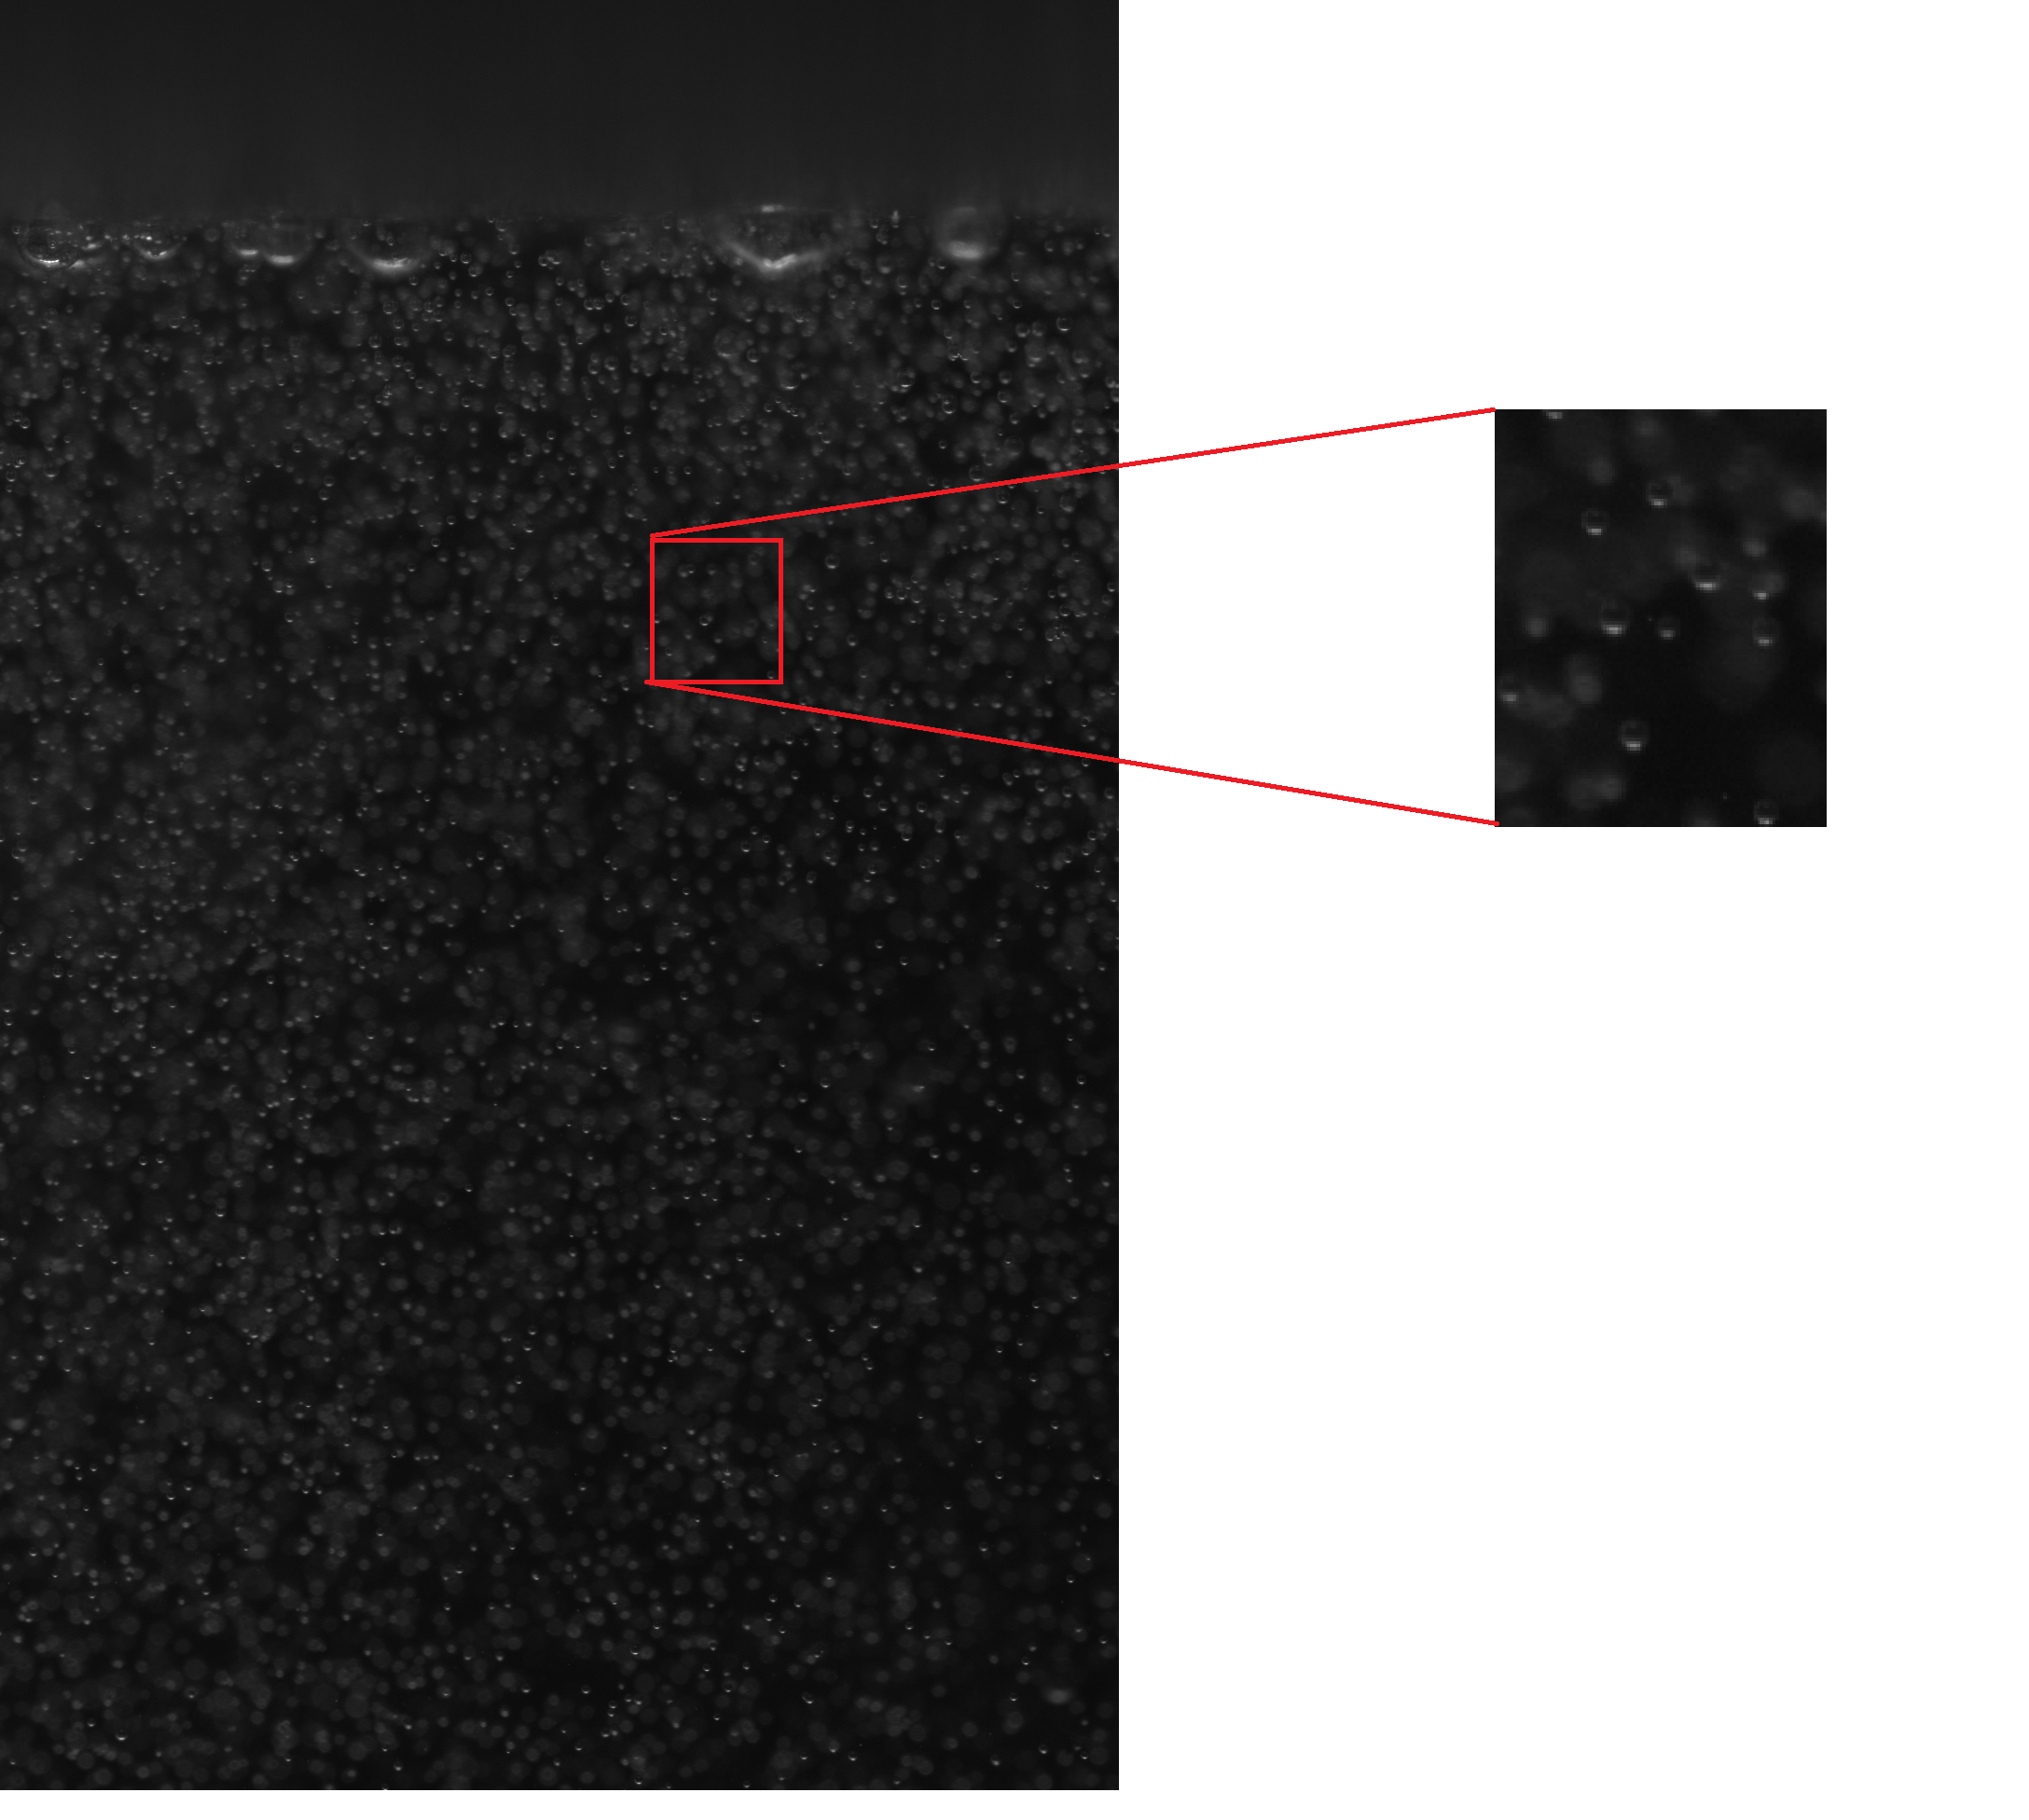
\includegraphics[scale=0.4]{images/aquarium_result_surf.png}
	\caption{Image captured close to the water surface with the aquarium setup. Most bubbles show the expected two peaks, except for those very close to the water surface, where bubble curvatures is also visible.}
\end{figure}

\begin{figure}
	\centering
	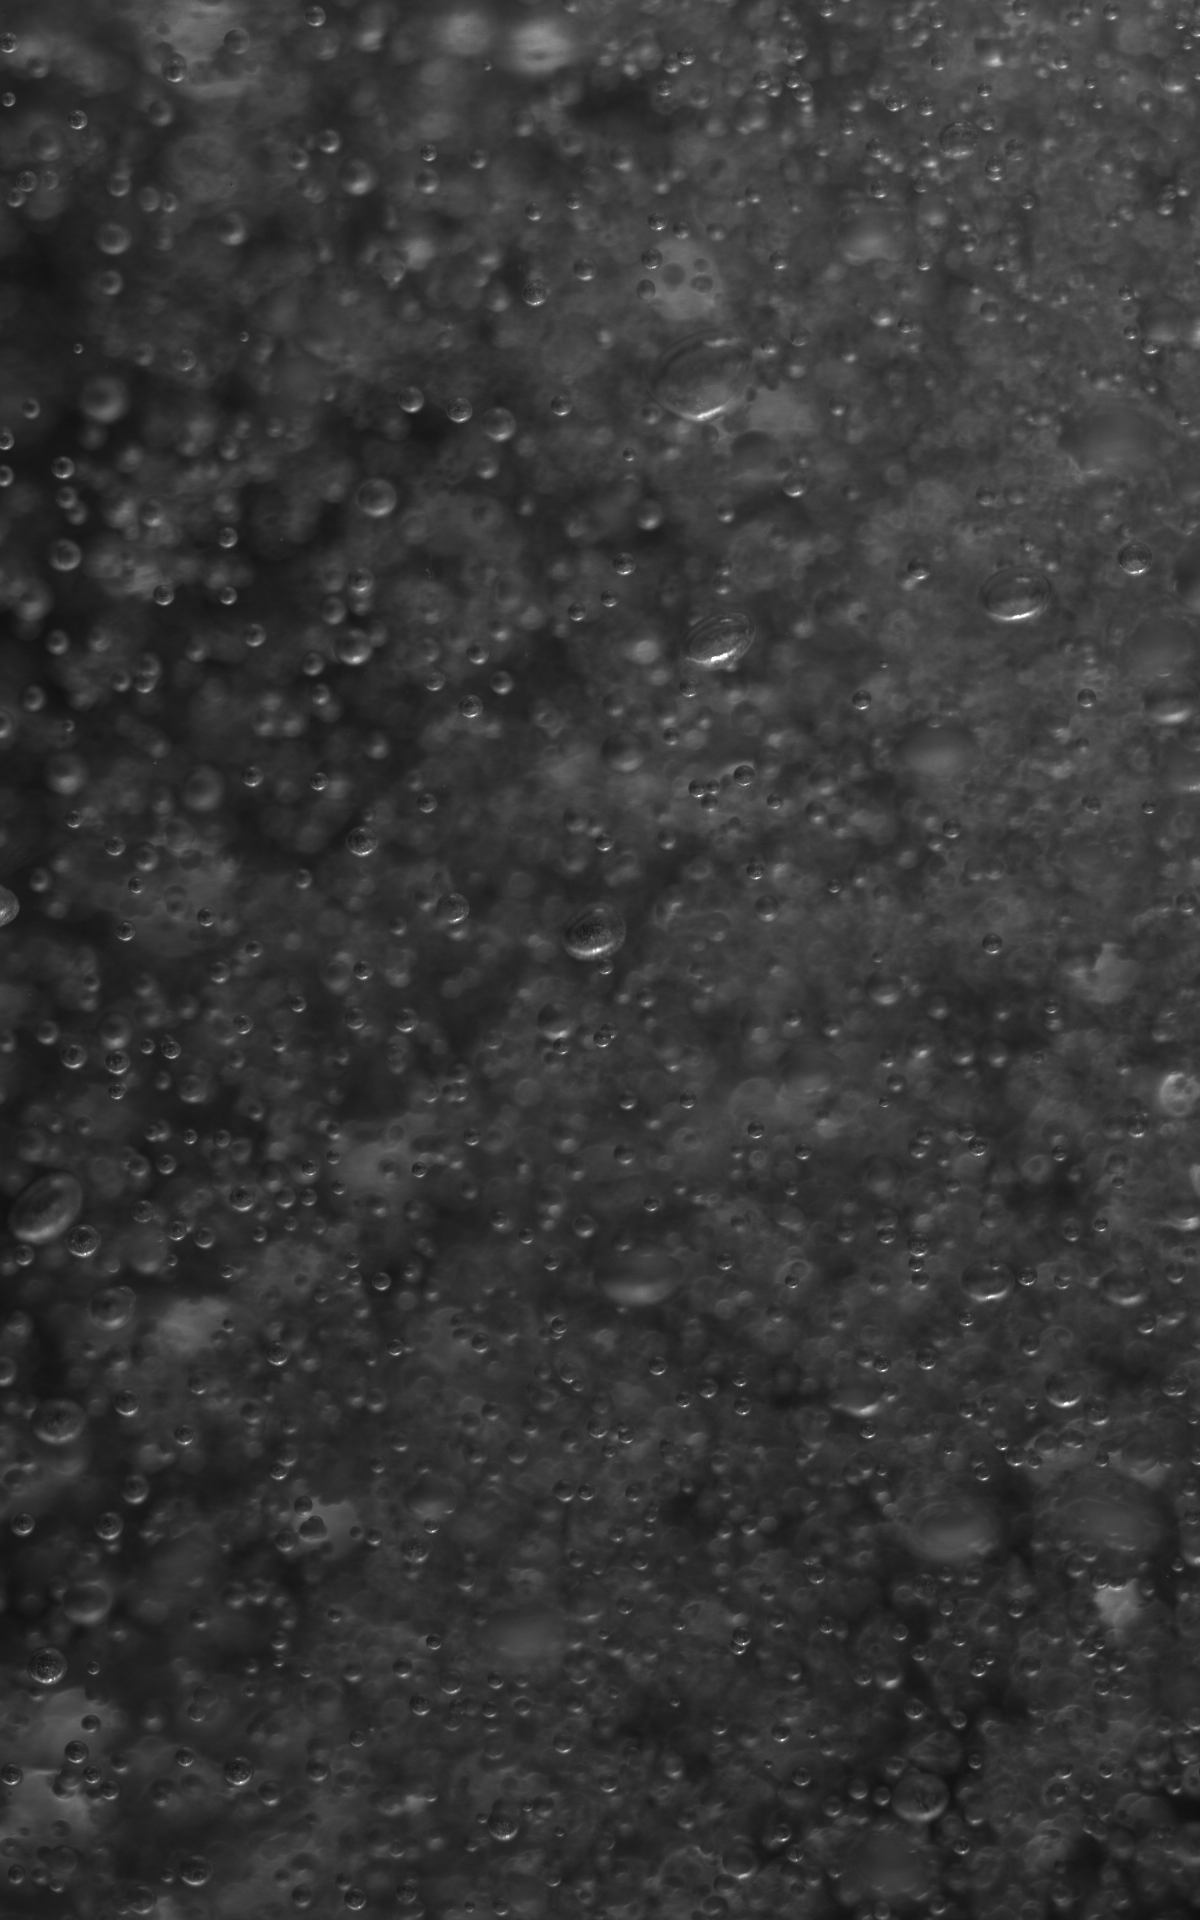
\includegraphics[scale=0.3]{images/aquarium_result_high_conc.jpg}
	\caption{Image with high bubble concentration at aquarium setup using a bubble generator.}
\end{figure}


\begin{figure}
	\centering
	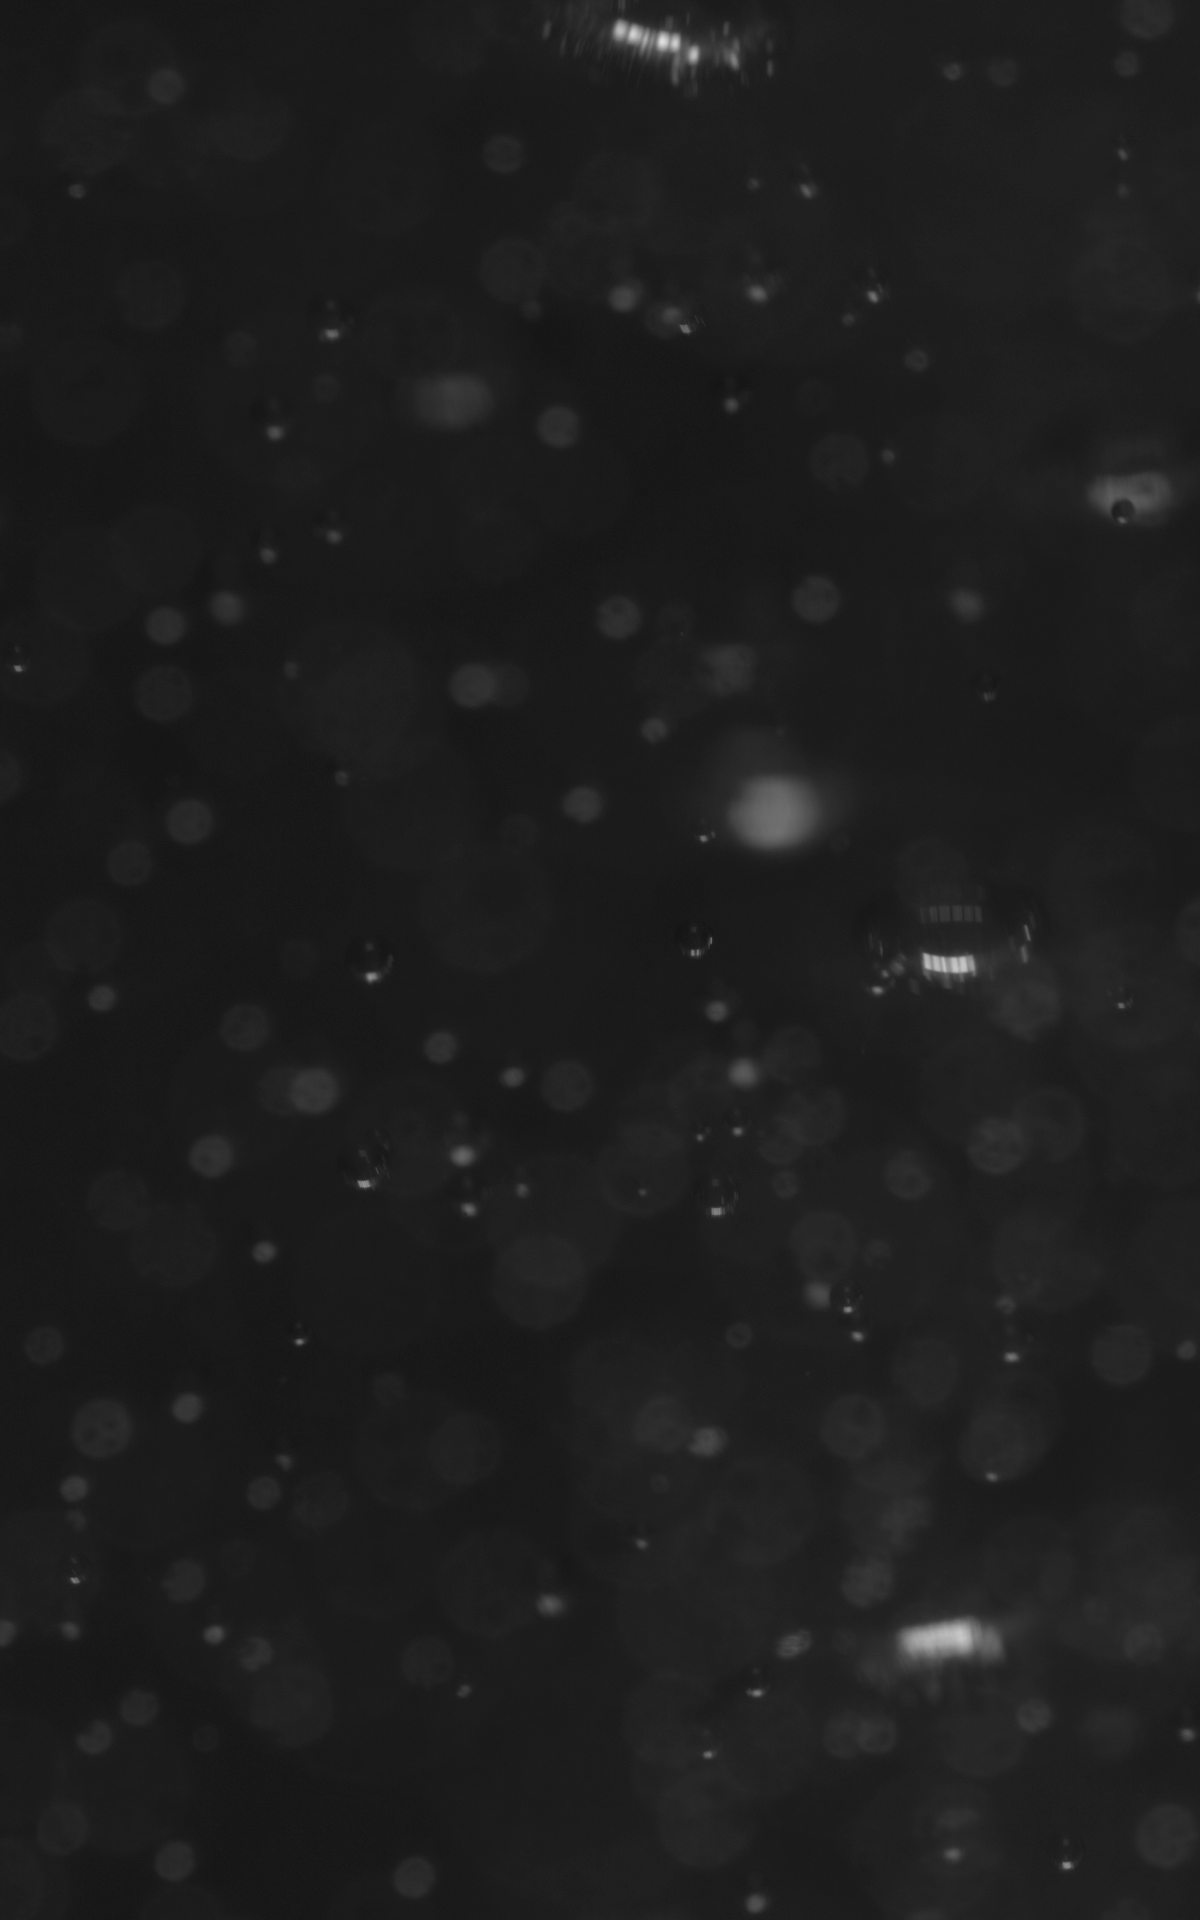
\includegraphics[scale=0.3]{images/aeolotron_result_raw.bmp}
	\caption{Image from Aeolotron setup with low bubble concentrations. Motion blur can be observed for larger bubbles moving fast.}
\end{figure}